\documentclass[twocolumn,a4j]{jsarticle}
\setlength{\topmargin}{-20.4cm}
\setlength{\oddsidemargin}{-10.4mm}
\setlength{\evensidemargin}{-10.4mm}
\setlength{\textwidth}{18cm}
\setlength{\textheight}{26cm}

\usepackage[top=15truemm,bottom=25truemm,left=15truemm,right=15truemm]{geometry}
\usepackage[latin1]{inputenc}
\usepackage{amsmath}
\usepackage{amsfonts}
\usepackage{amssymb}
\usepackage[dvipdfmx]{graphicx}
\usepackage[dvipdfmx]{color}
\usepackage{listings}
\usepackage{listings,jvlisting}
\usepackage{geometry}
\usepackage{framed}
\usepackage{color}
\usepackage[dvipdfmx]{hyperref}
\usepackage{ascmac}
\usepackage{enumerate}
\usepackage{tabularx}
\usepackage{cancel}
\usepackage{scalefnt}

\renewcommand{\figurename}{Fig.}
\renewcommand{\tablename}{Table }

\lstset{
basicstyle={\ttfamily},
identifierstyle={\small},
commentstyle={\smallitshape},
keywordstyle={\small\bfseries},
ndkeywordstyle={\small},
stringstyle={\small\ttfamily},
frame={tb},
breaklines=true,
columns=[l]{fullflexible},
xrightmargin=0zw,
xleftmargin=3zw,
numberstyle={\scriptsize},
stepnumber=1,
numbersep=1zw,
lineskip=-0.5ex
}

\makeatletter
\def\@maketitle
{
\begin{center}
{\LARGE \@title \par}
\end{center}
\begin{flushright}
{\large 報告書 NO.08 - 2\quad\@date\quad\@author}
\end{flushright}
\par\vskip 1.5em
}
\makeatother

\setcounter{tocdepth}{3}

\author{来代 勝胤}
\title{令和3年度 12月 第3週 報告書}
\date{2021/12/16}

\begin{document}
\columnseprule=0.1mm

\maketitle
\section*{報告内容}
\begin{enumerate}[1.]
    \item 進捗状況
    \item 模擬実験結果
\end{enumerate}

\section{進捗状況}
今週は,引き続き模擬実験を行った。
また,その実験結果のデータ処理を行った。

\section{模擬実験}

先週に引き続き実験を行った。
実験結果のまとめを以下のTable.1及びFig.1、Fig.2に示す。
また、角度における実験結果を以下に示す。

\begin{table}[htbp]
    \begin{center}
        \caption{Summary of value}
        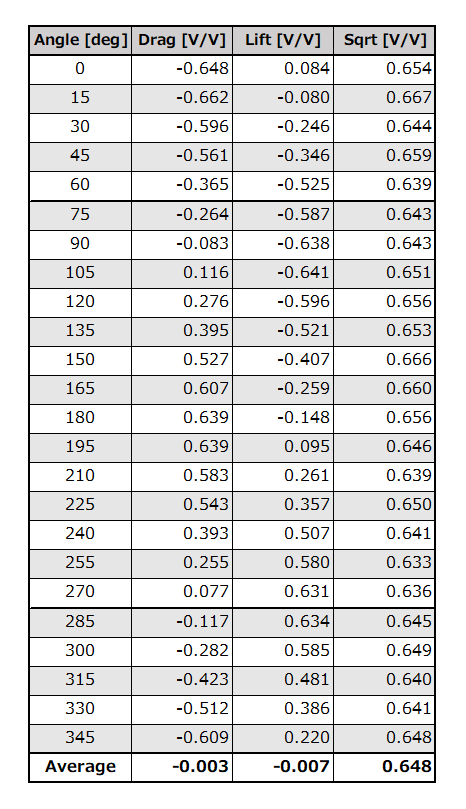
\includegraphics[width=82mm]{../images/table_1.png}
    \end{center}
\end{table}

\begin{figure}[htbp]
    \footnotesize
    \begin{center}
        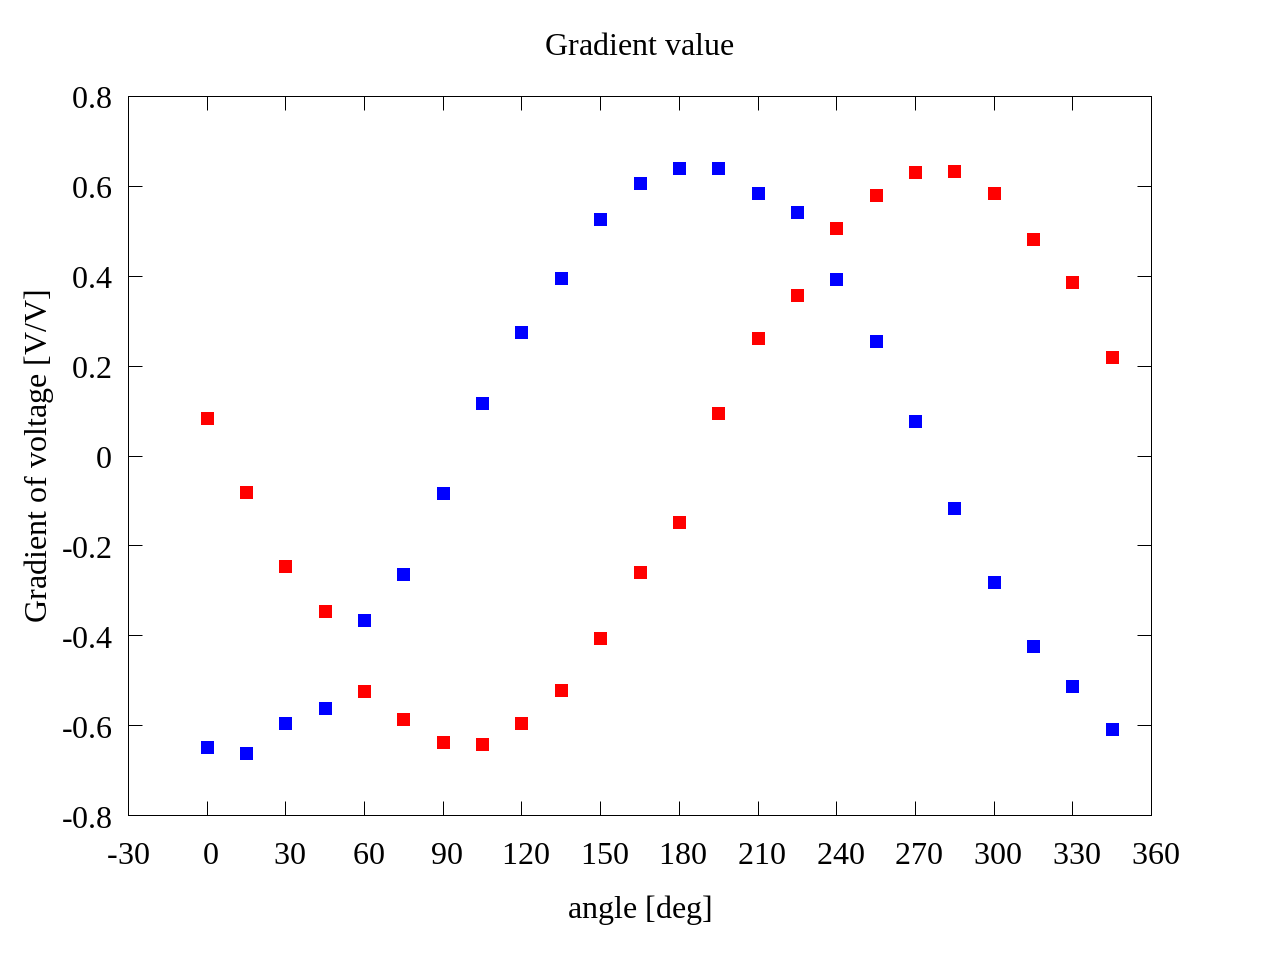
\includegraphics[width=85mm]{../images/summary/summary_1.png}
        \caption{Summary of gradient value}
        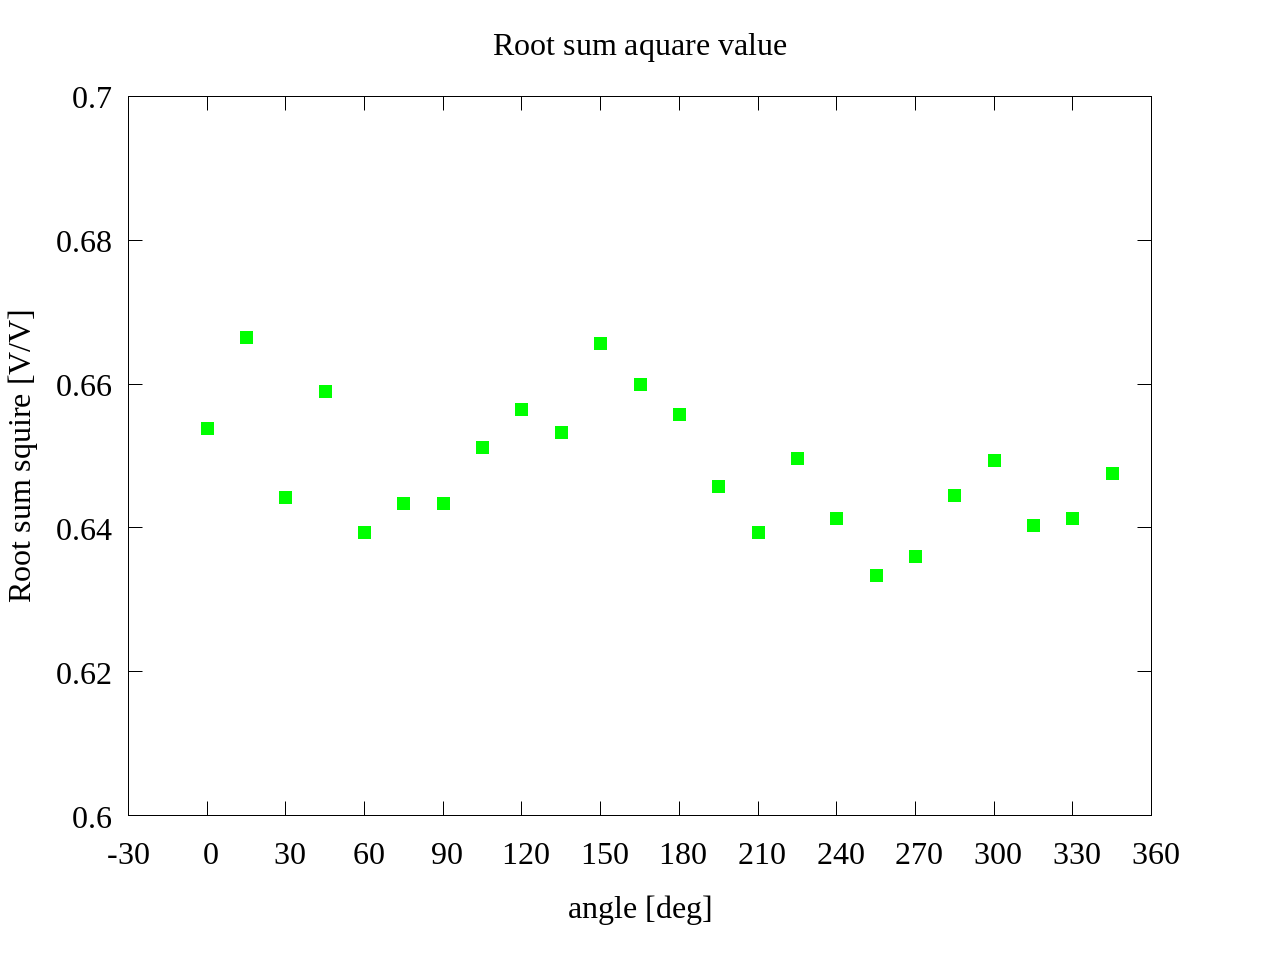
\includegraphics[width=85mm]{../images/summary/summary_2.png}
        \caption{Summary of root sum square value}
    \end{center}
\end{figure}

\begin{figure}[htbp]
    \footnotesize
    \begin{center}
        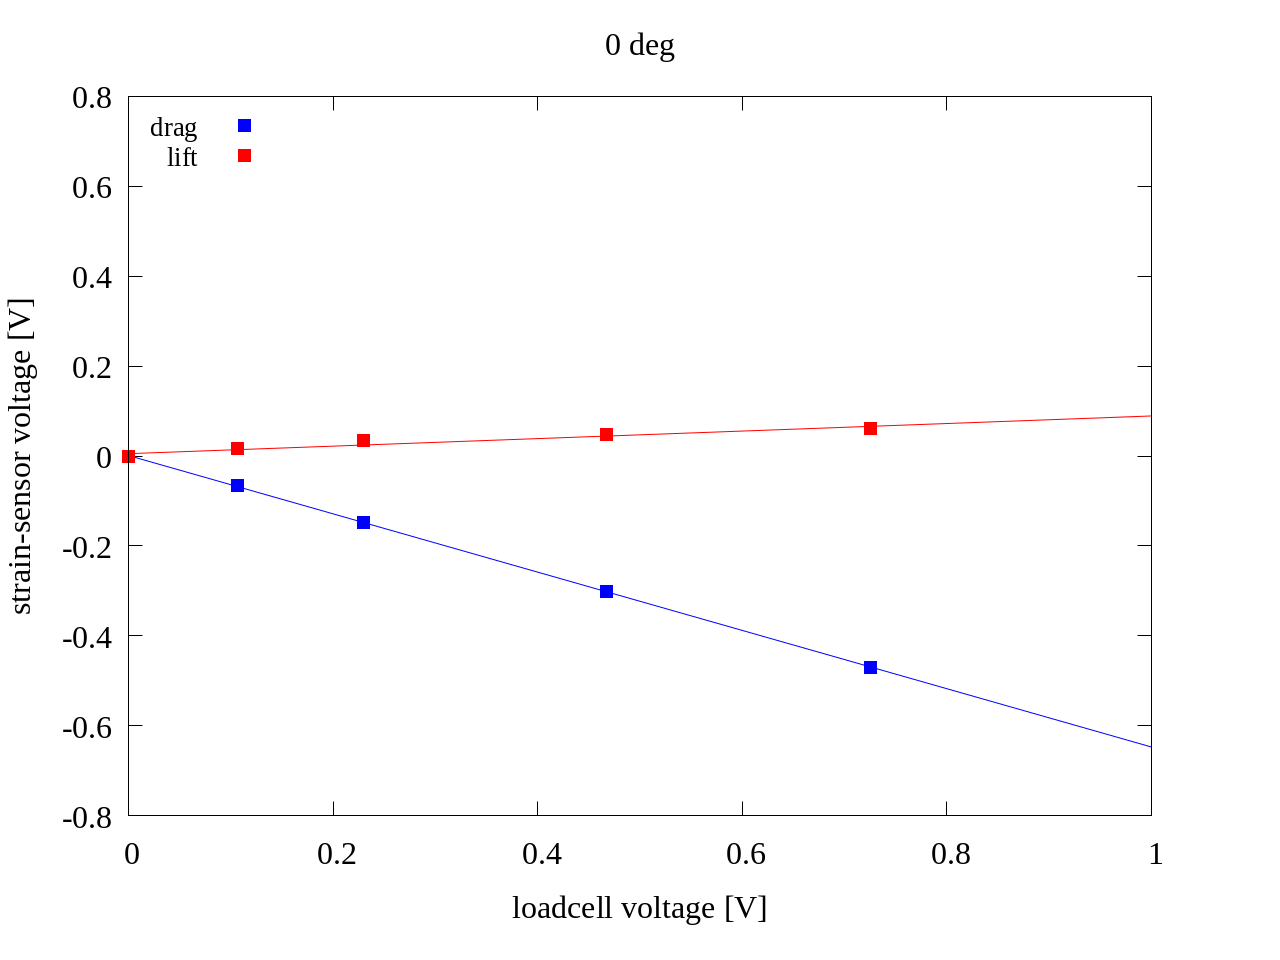
\includegraphics[width=78mm]{../images/linear/0_linear.png}
        \caption{0 deg}
        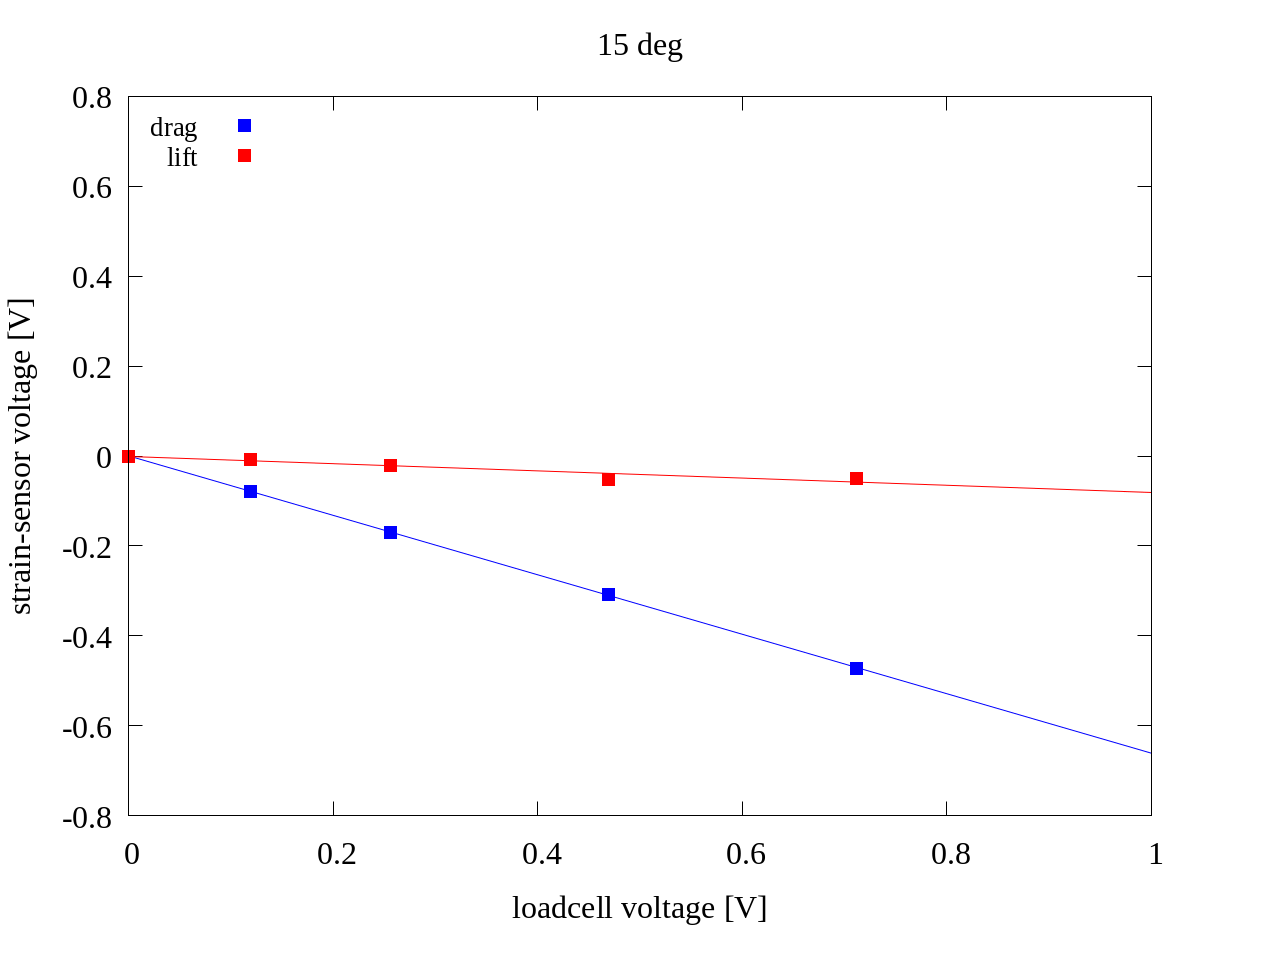
\includegraphics[width=78mm]{../images/linear/15_linear.png}
        \caption{15 deg}
        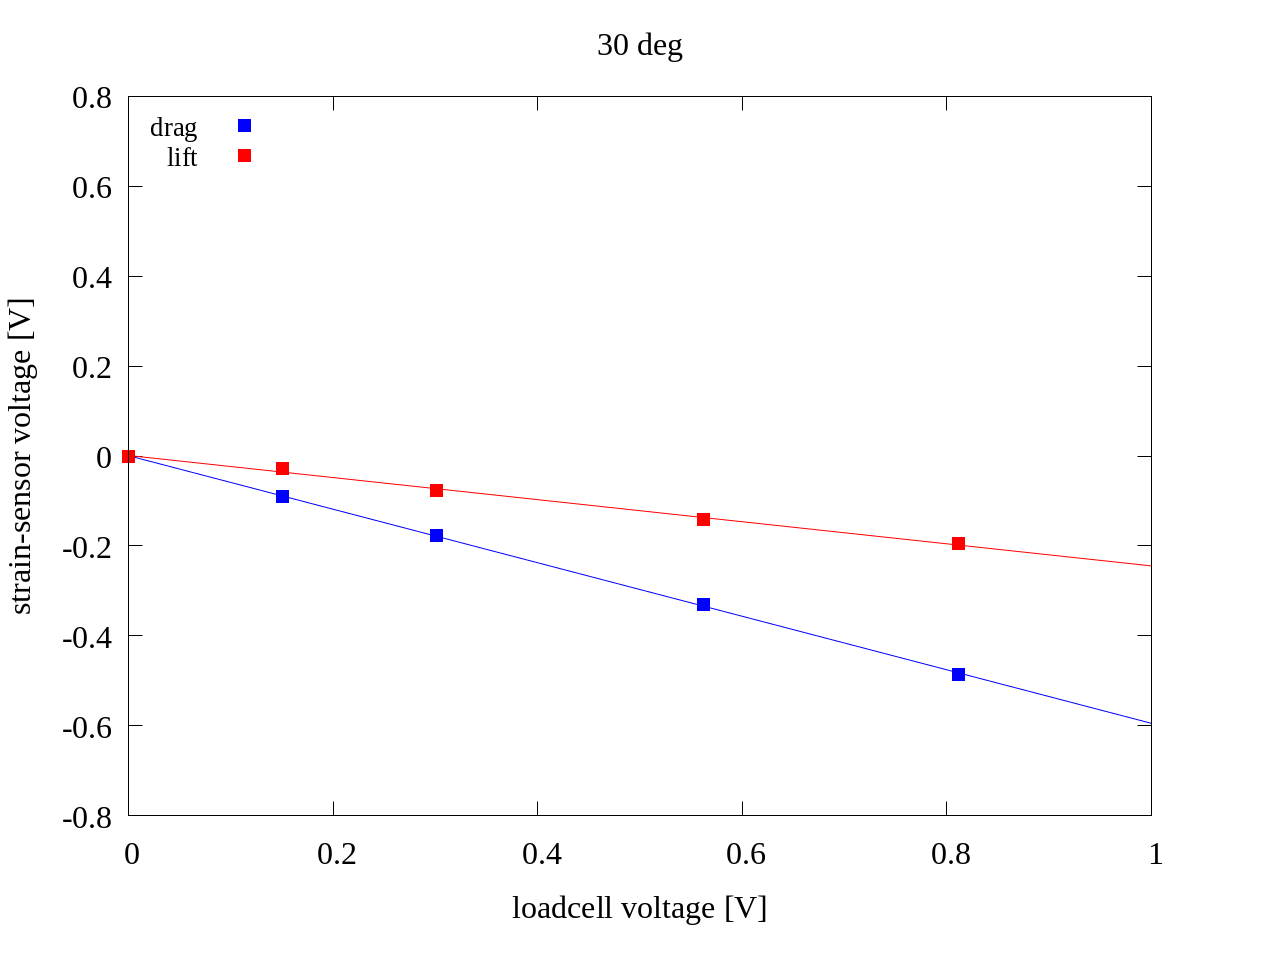
\includegraphics[width=78mm]{../images/linear/30_linear.png}
        \caption{30 deg}
        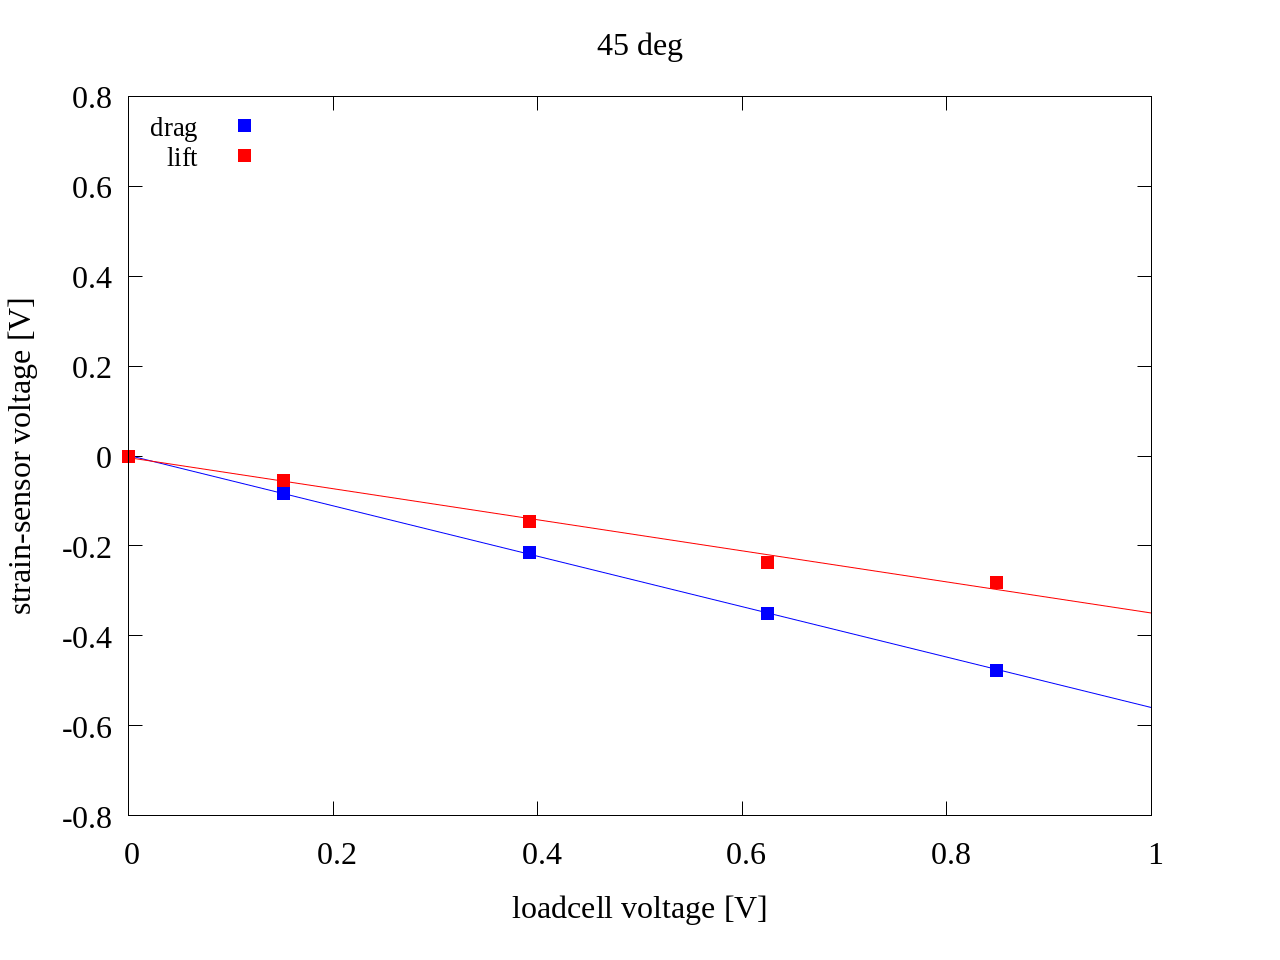
\includegraphics[width=78mm]{../images/linear/45_linear.png}
        \caption{45 deg}
    \end{center}
\end{figure}

\par
\newpage

\begin{figure}[htbp]
    \footnotesize
    \begin{center}
        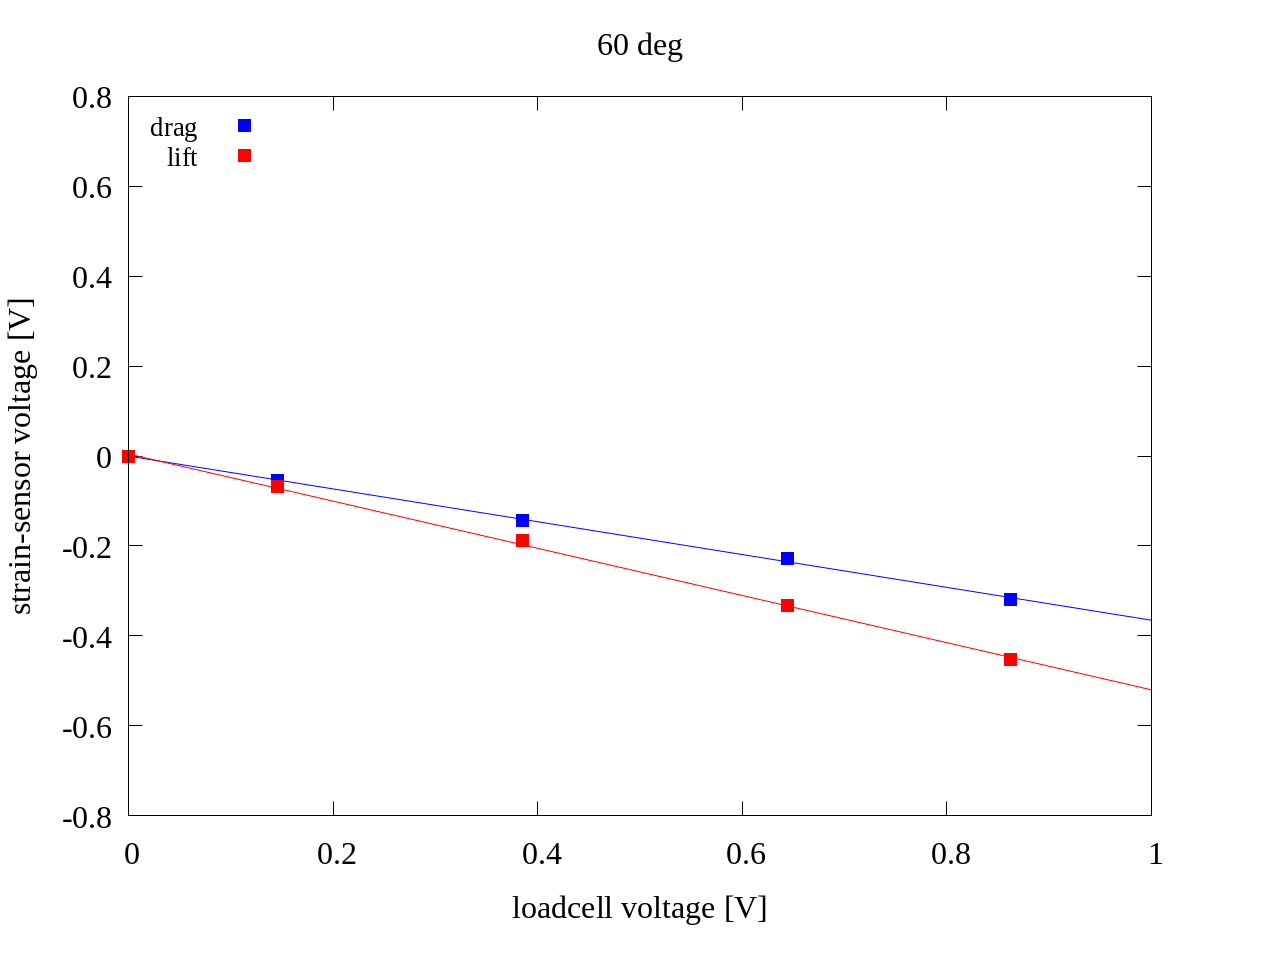
\includegraphics[width=78mm]{../images/linear/60_linear.png}
        \caption{60 deg}
        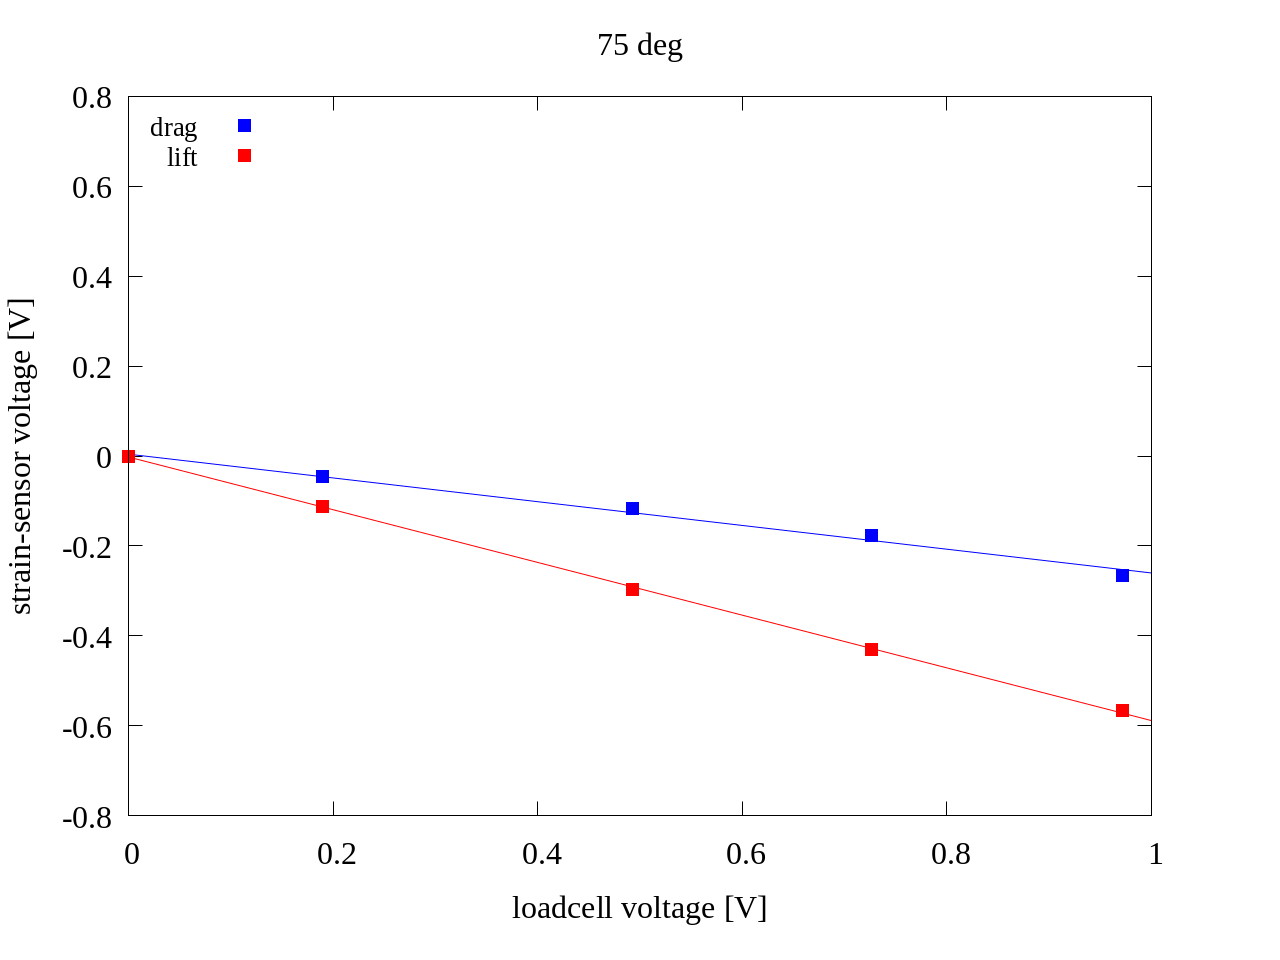
\includegraphics[width=78mm]{../images/linear/75_linear.png}
        \caption{75 deg}
        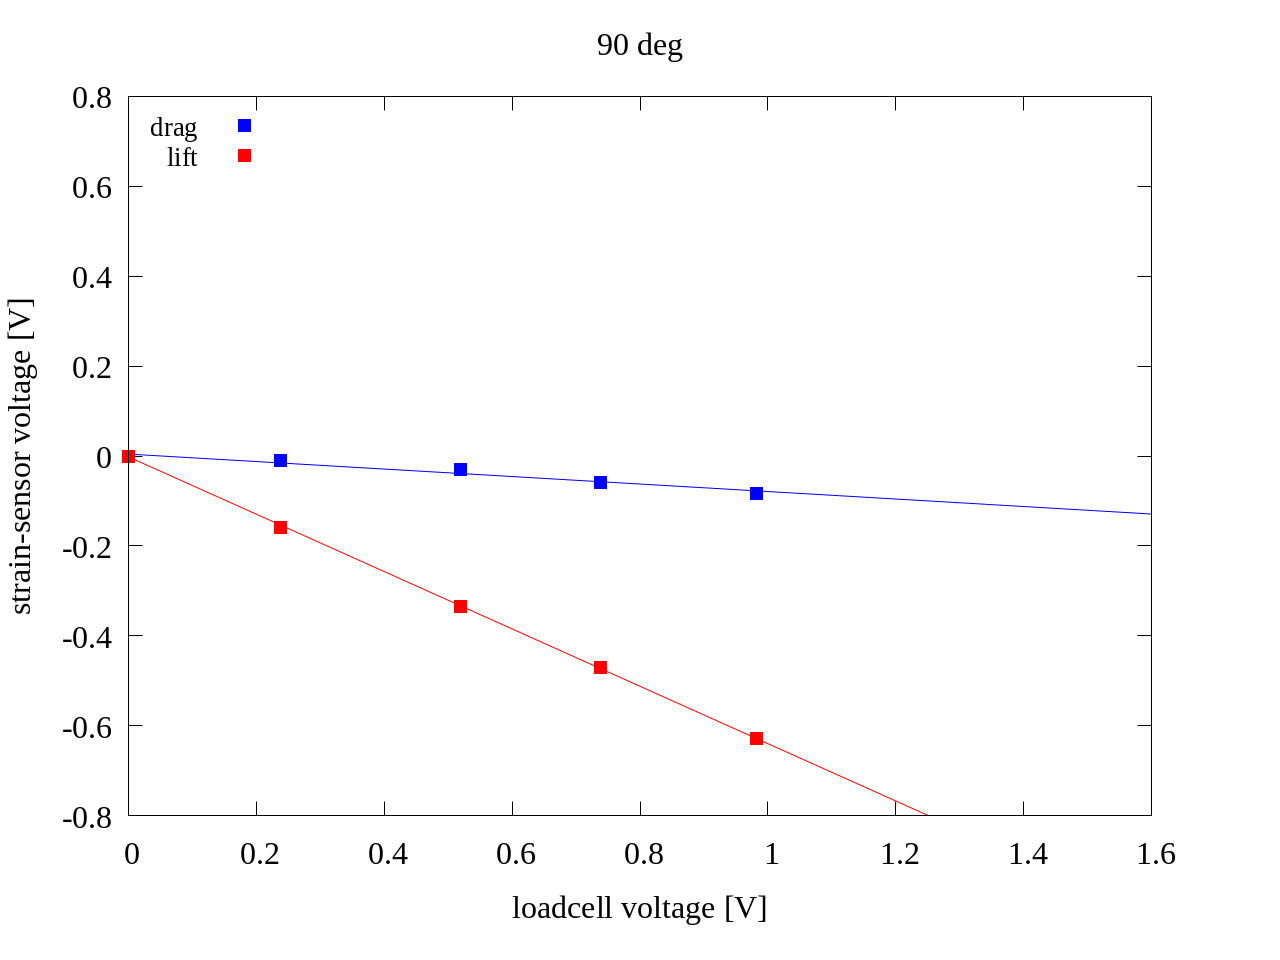
\includegraphics[width=78mm]{../images/linear/90_linear.png}
        \caption{90 deg}
        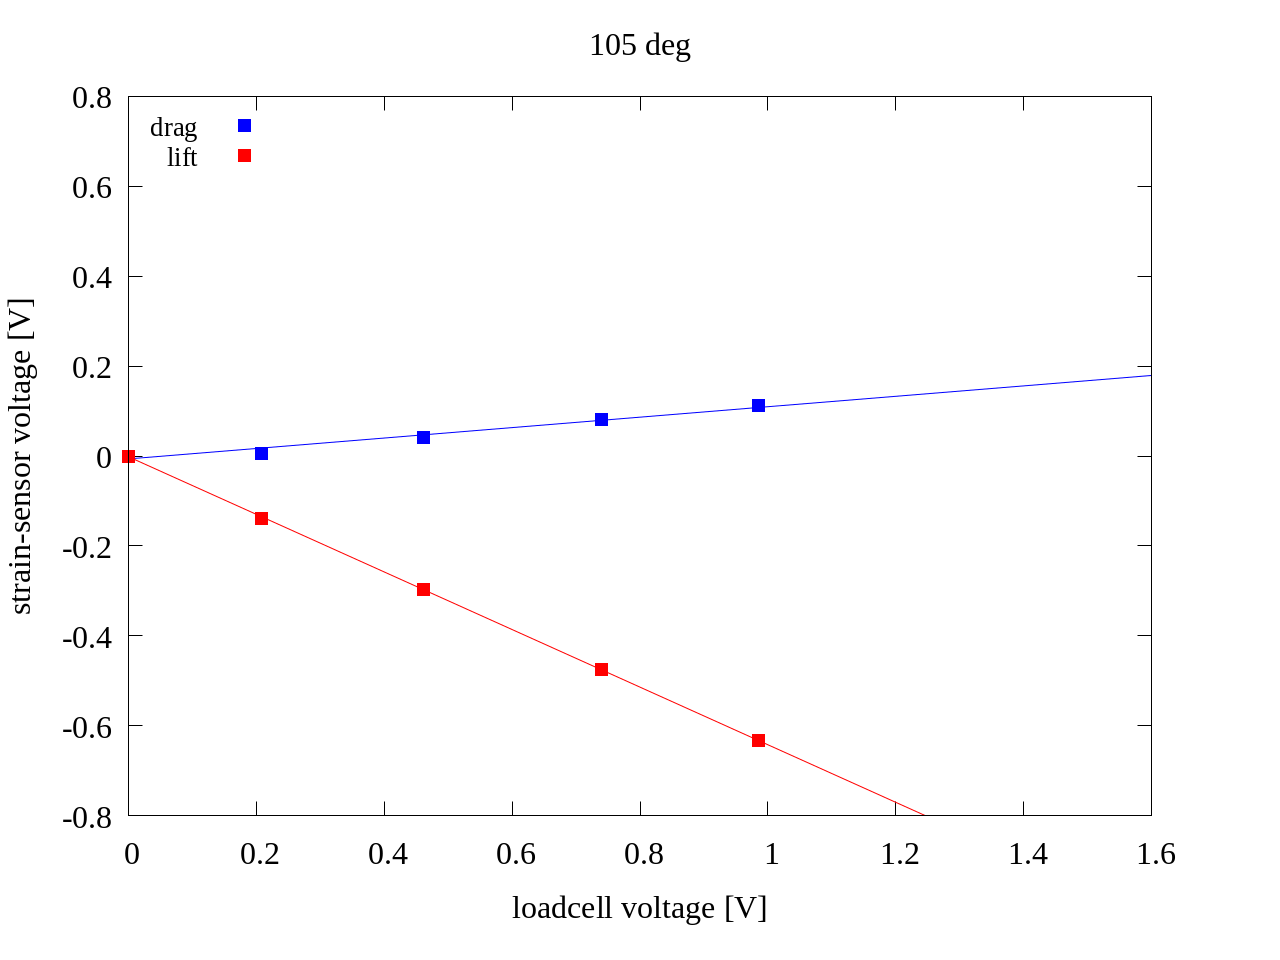
\includegraphics[width=78mm]{../images/linear/105_linear.png}
        \caption{105 deg}
    \end{center}
\end{figure}

\par
\newpage

\begin{figure}[htbp]
    \footnotesize
    \begin{center}
        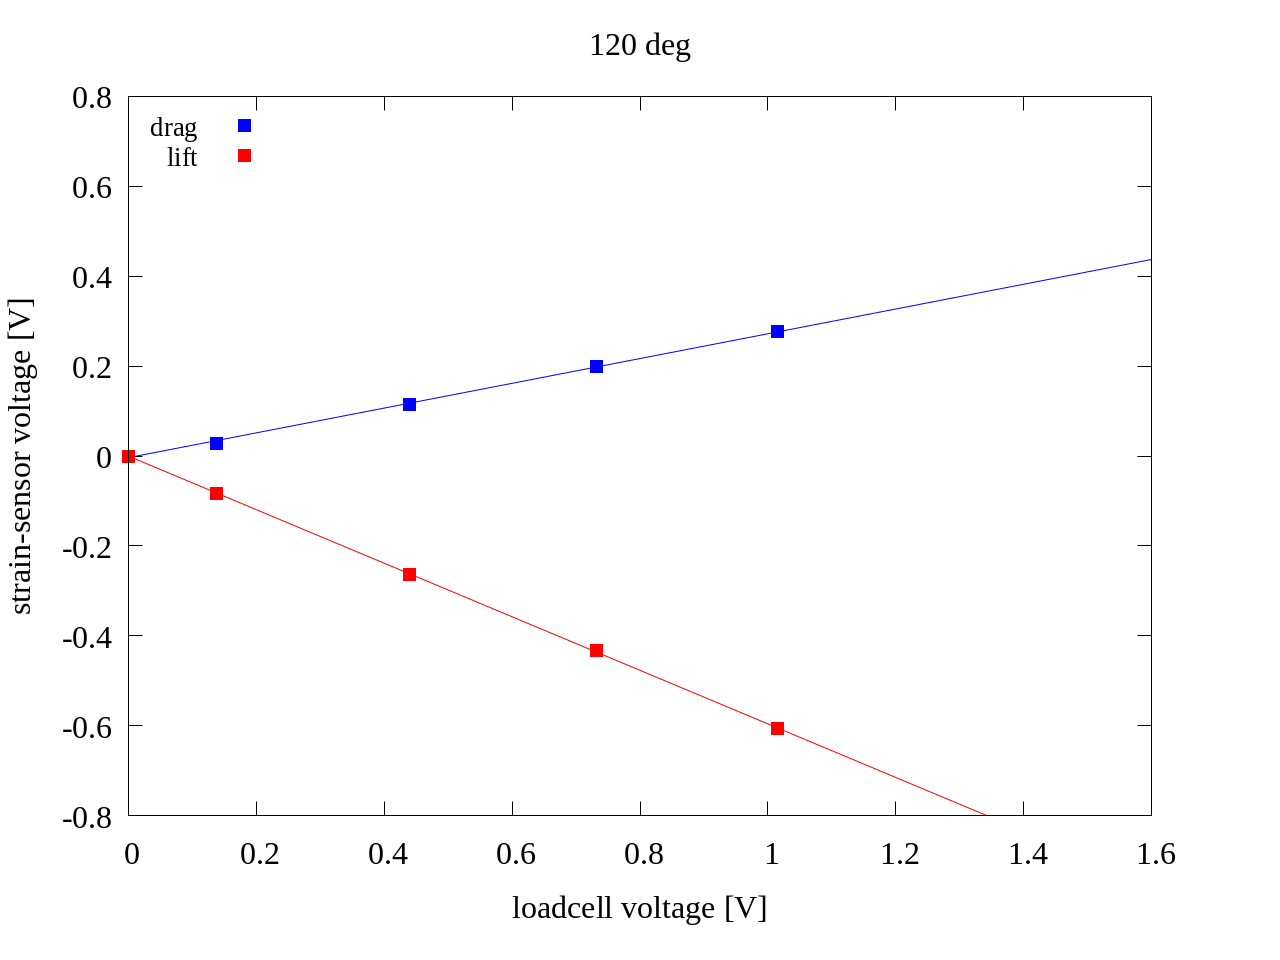
\includegraphics[width=78mm]{../images/linear/120_linear.png}
        \caption{120 deg}
        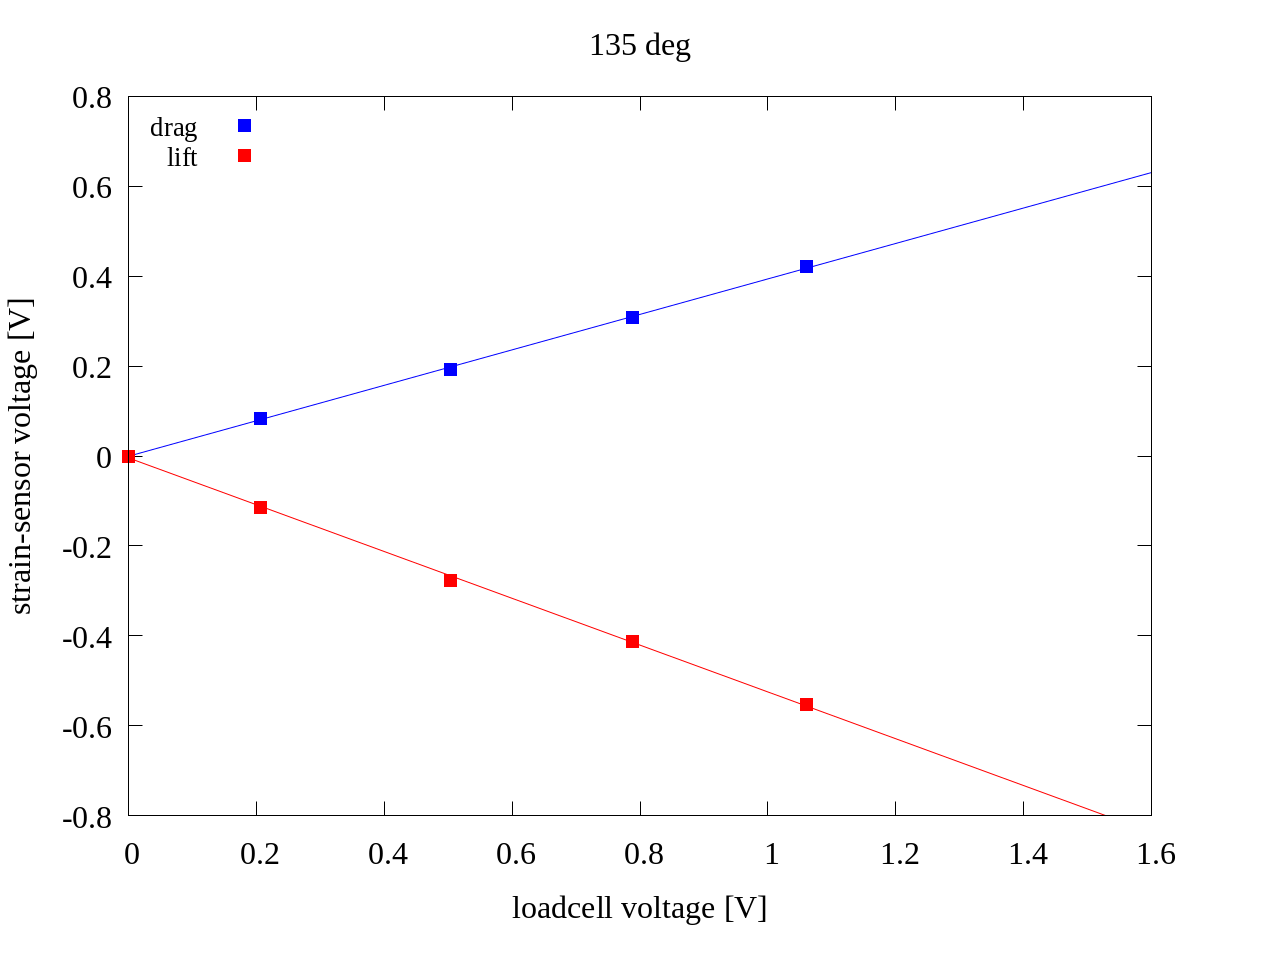
\includegraphics[width=78mm]{../images/linear/135_linear.png}
        \caption{135 deg}
        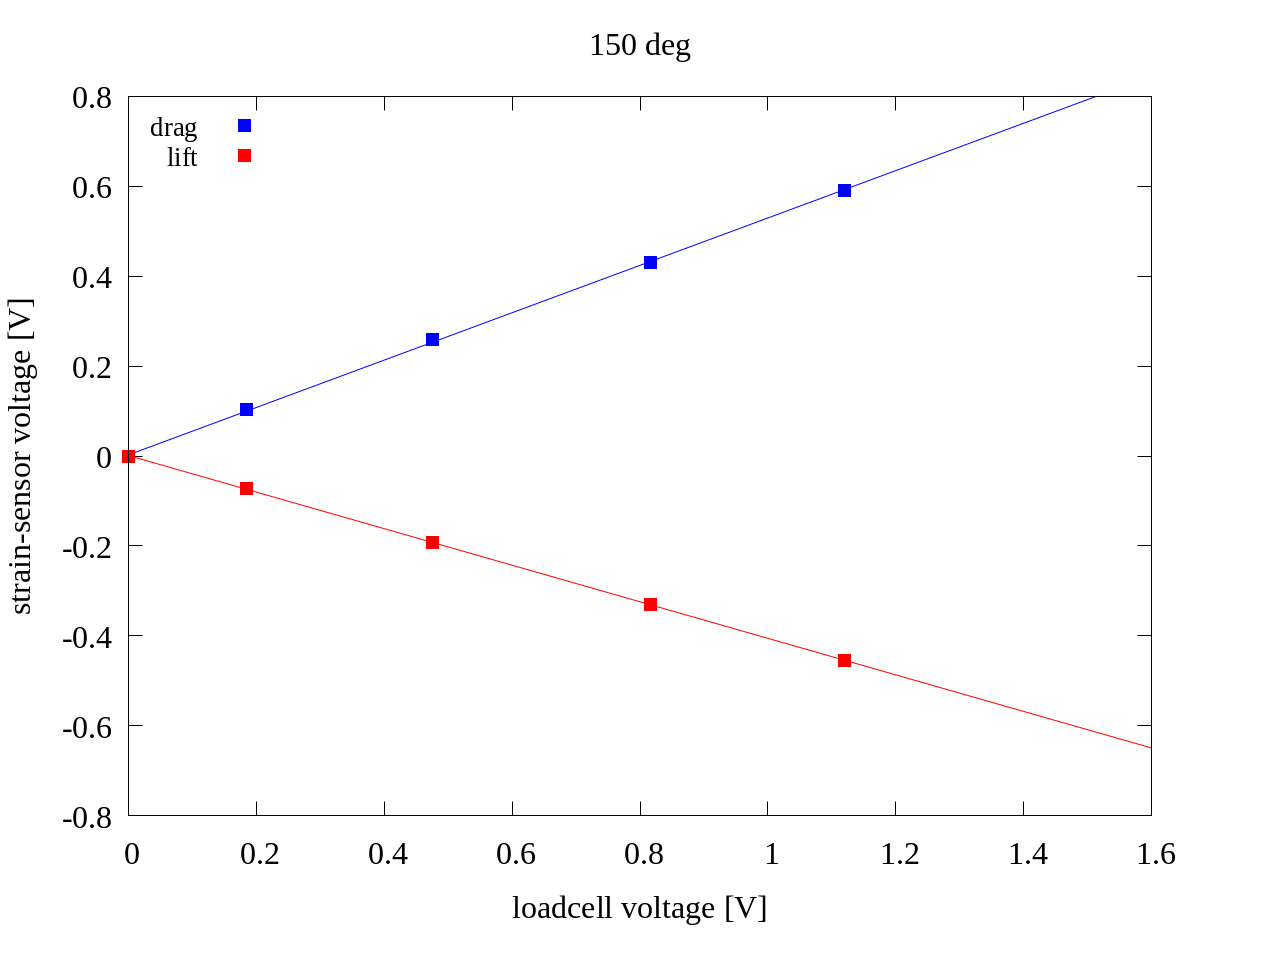
\includegraphics[width=78mm]{../images/linear/150_linear.png}
        \caption{150 deg}
        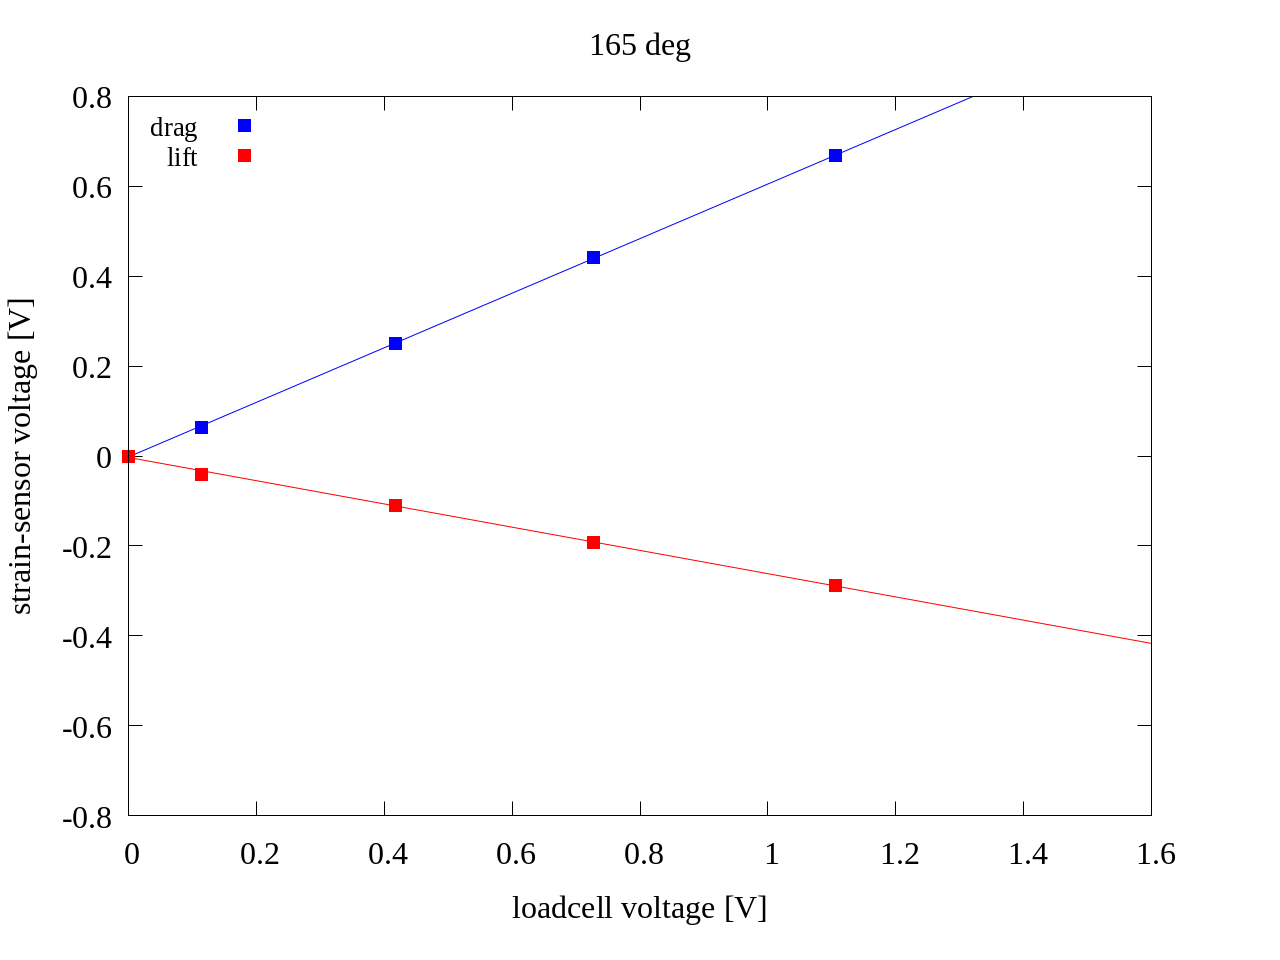
\includegraphics[width=78mm]{../images/linear/165_linear.png}
        \caption{165 deg}
    \end{center}
\end{figure}

\par
\newpage

\begin{figure}[htbp]
    \footnotesize
    \begin{center}
        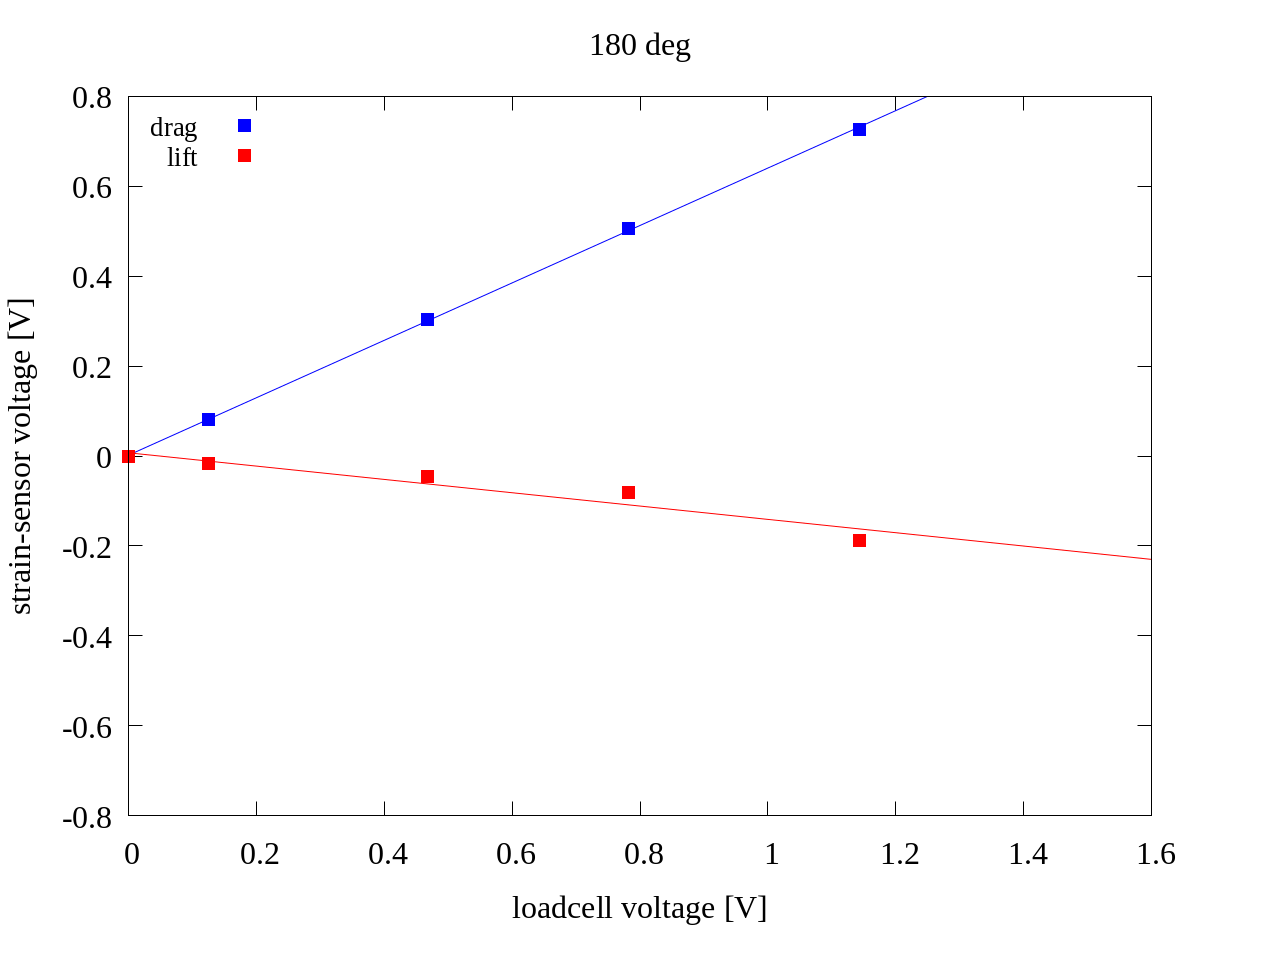
\includegraphics[width=78mm]{../images/linear/180_linear.png}
        \caption{180 deg}
        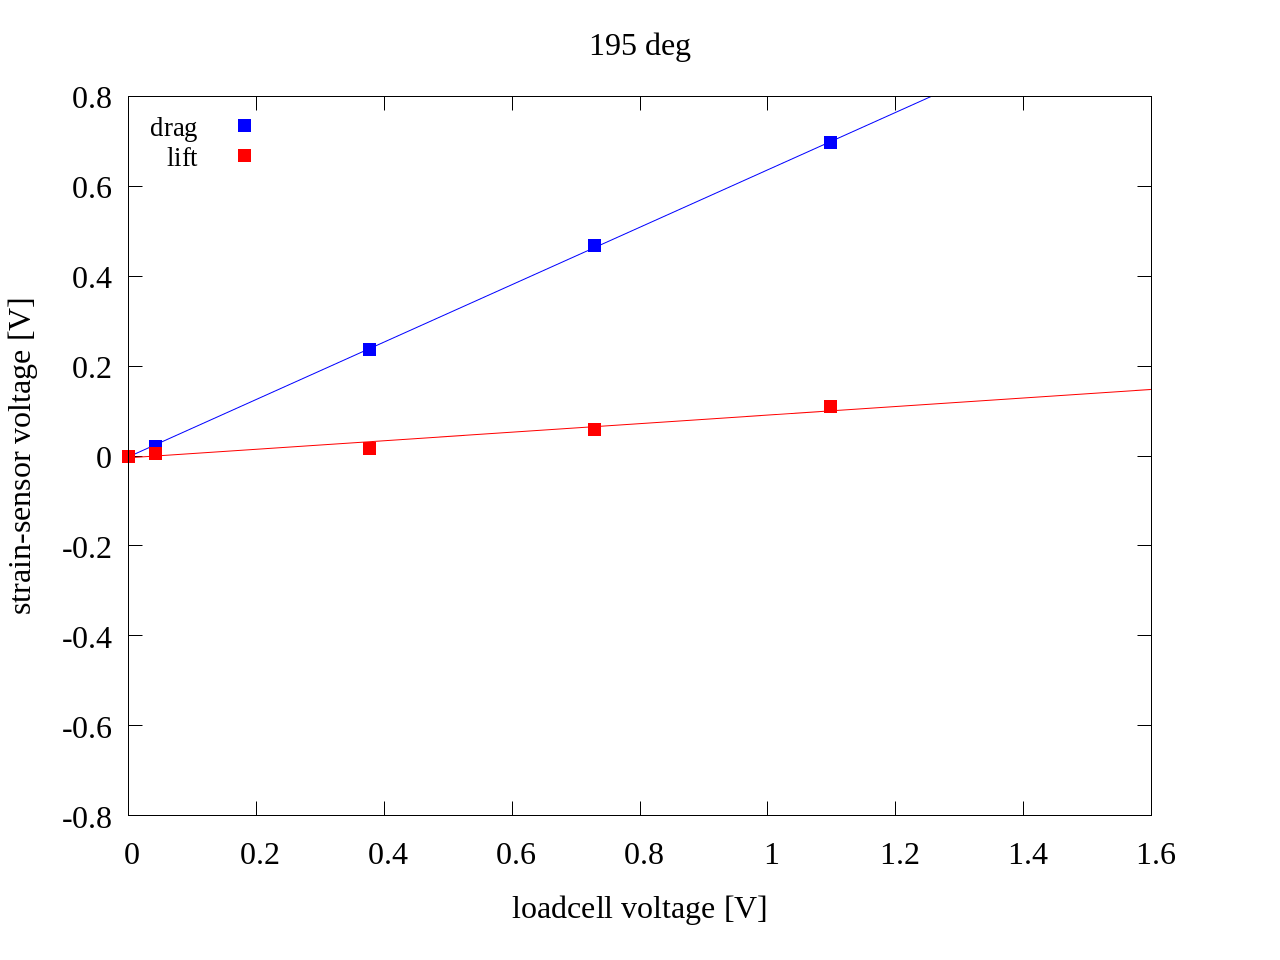
\includegraphics[width=78mm]{../images/linear/195_linear.png}
        \caption{195 deg}
        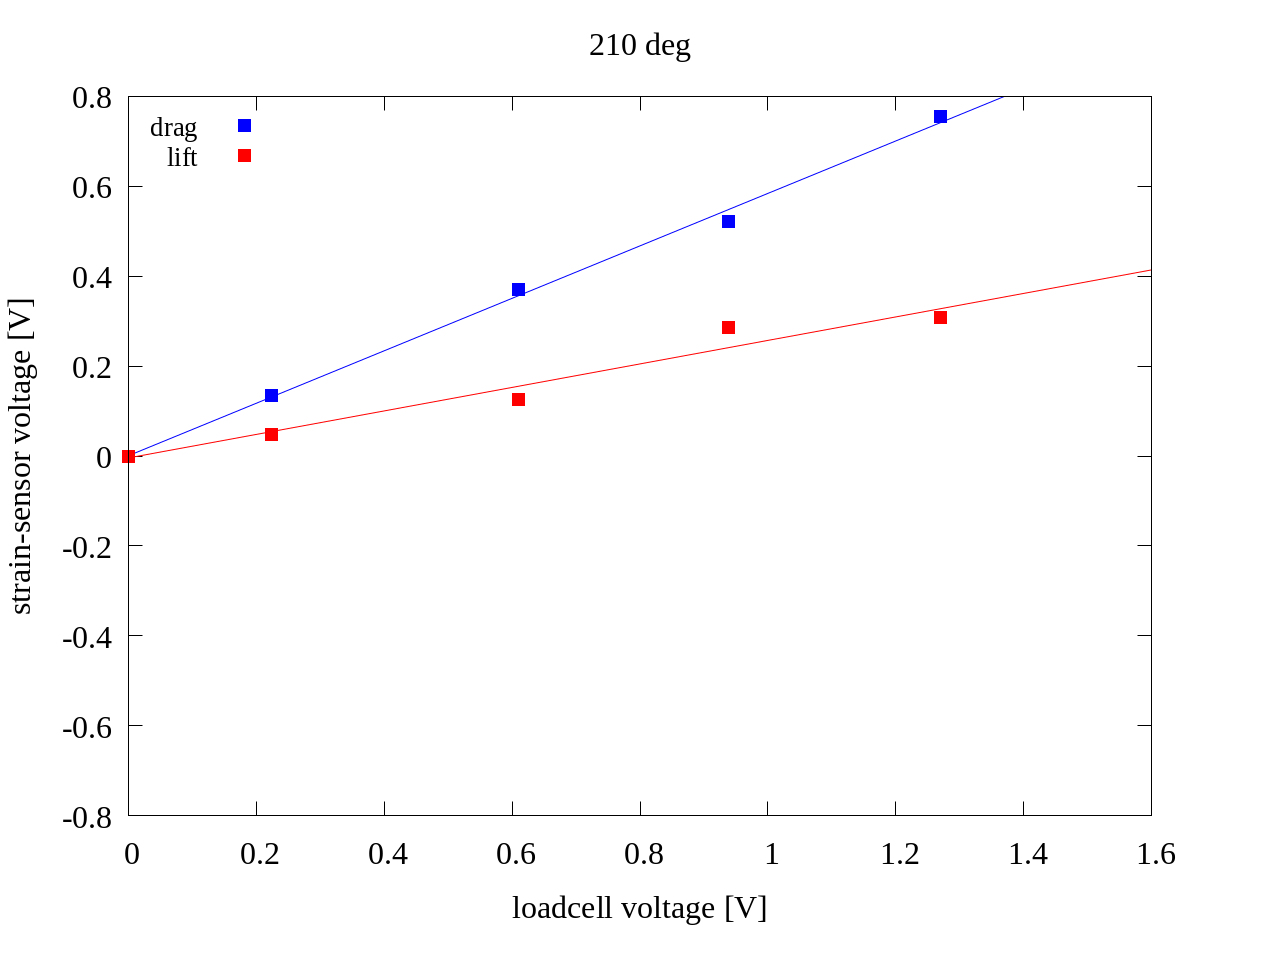
\includegraphics[width=78mm]{../images/linear/210_linear.png}
        \caption{210 deg}
        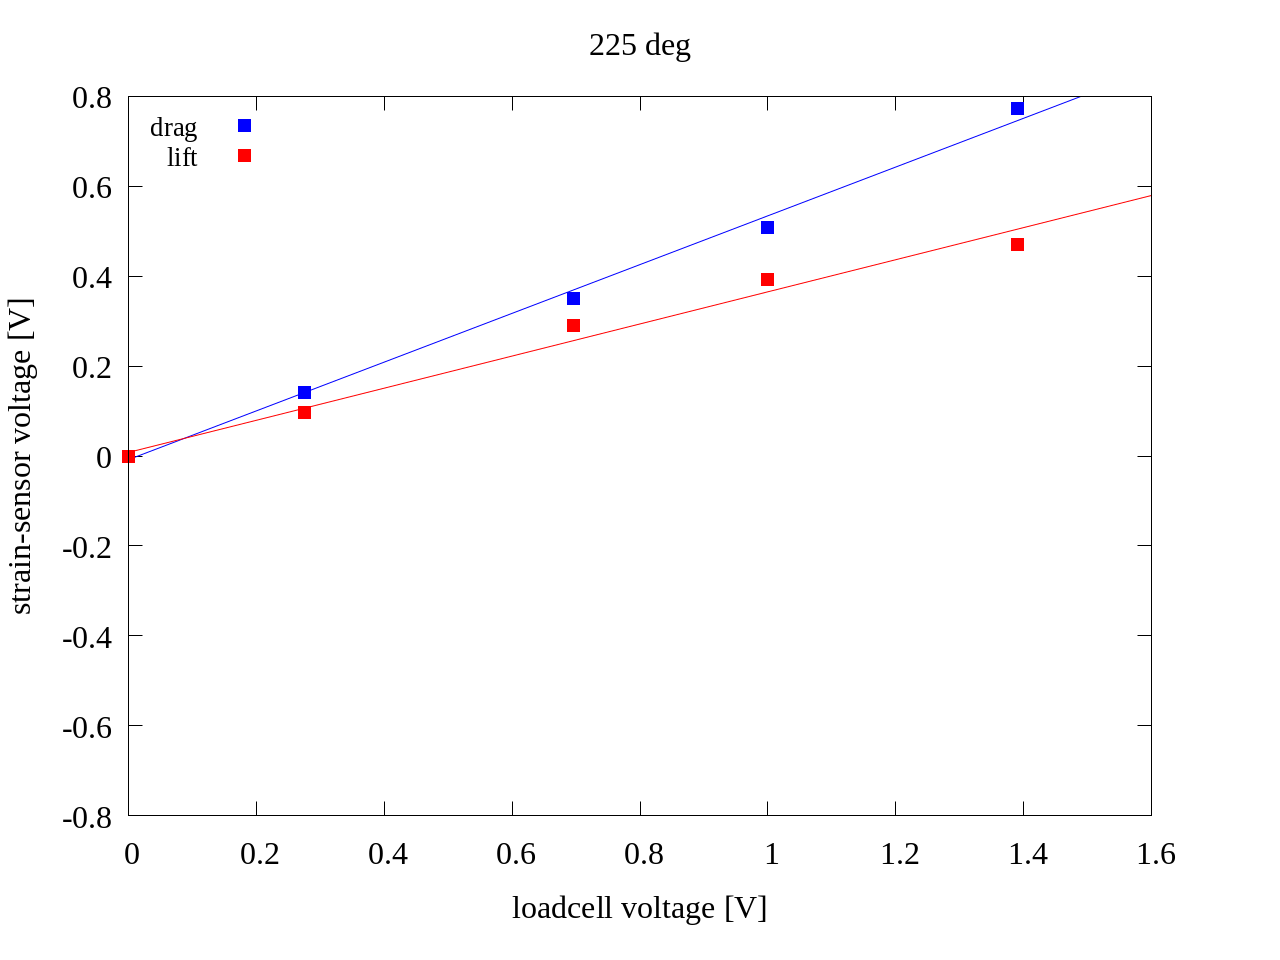
\includegraphics[width=78mm]{../images/linear/225_linear.png}
        \caption{225 deg}
    \end{center}
\end{figure}

\begin{figure}[htbp]
    \footnotesize
    \begin{center}
        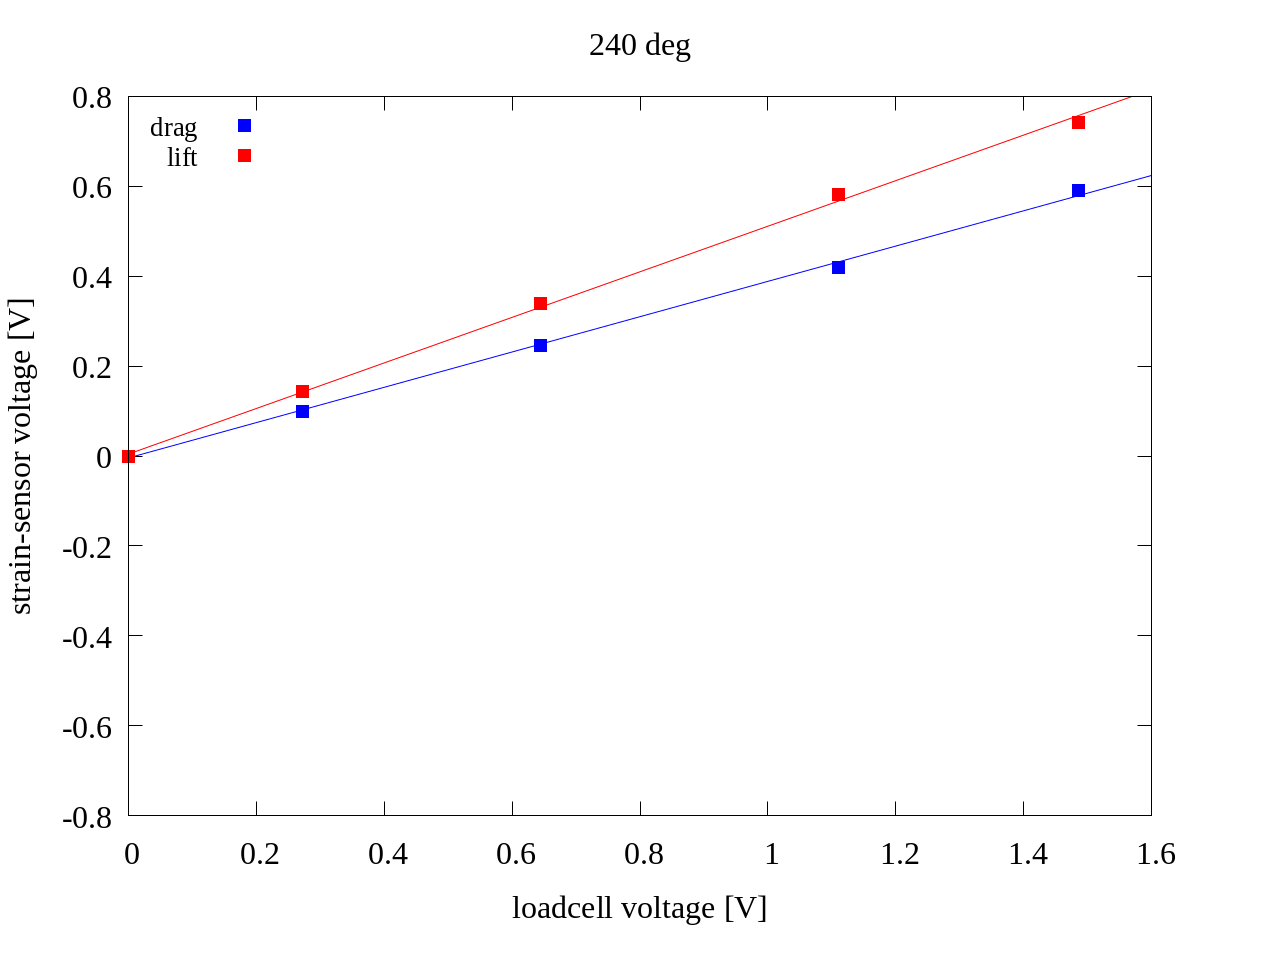
\includegraphics[width=78mm]{../images/linear/240_linear.png}
        \caption{240 deg}
        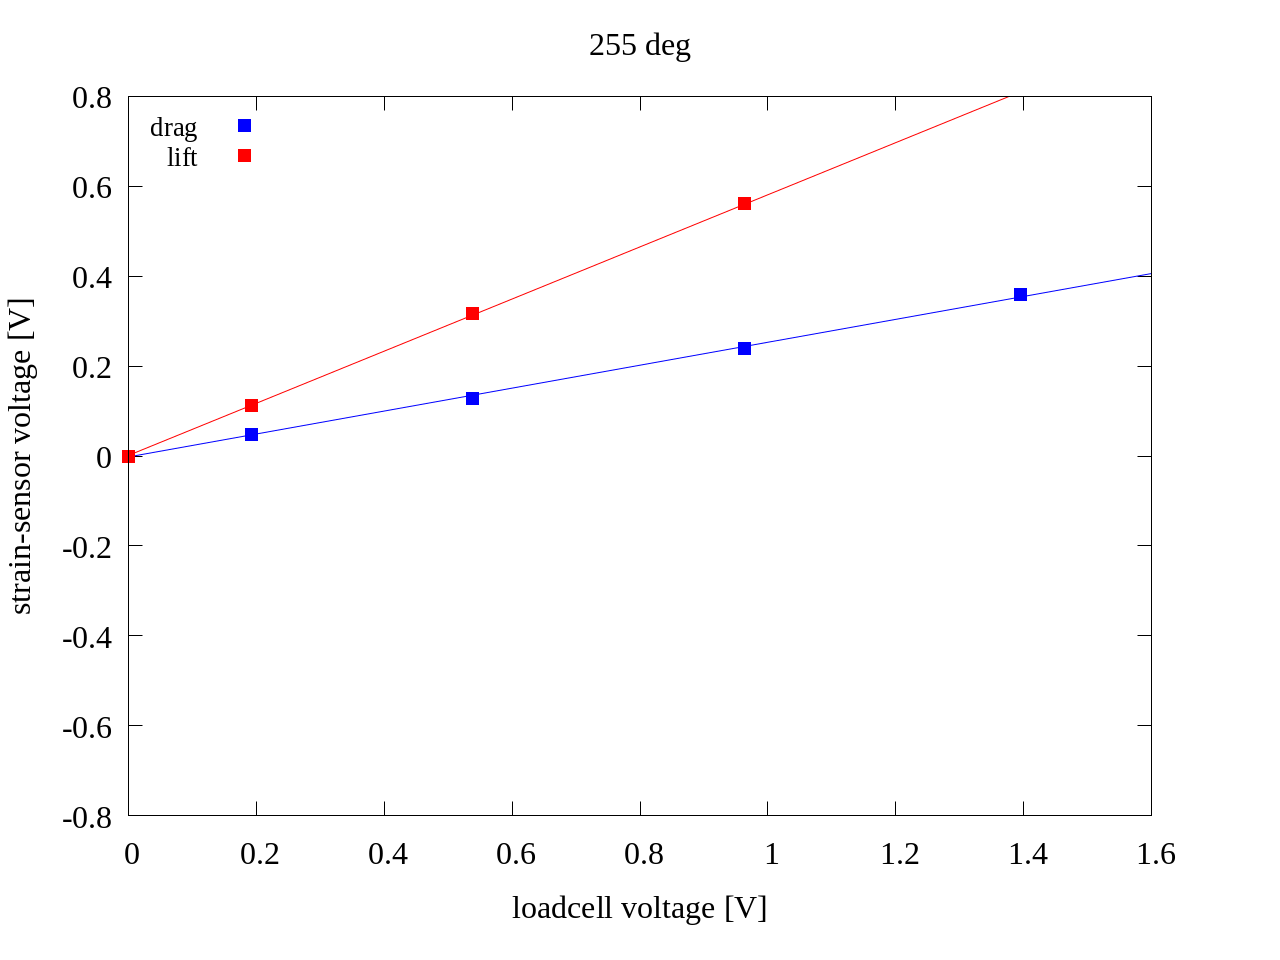
\includegraphics[width=78mm]{../images/linear/255_linear.png}
        \caption{255 deg}
        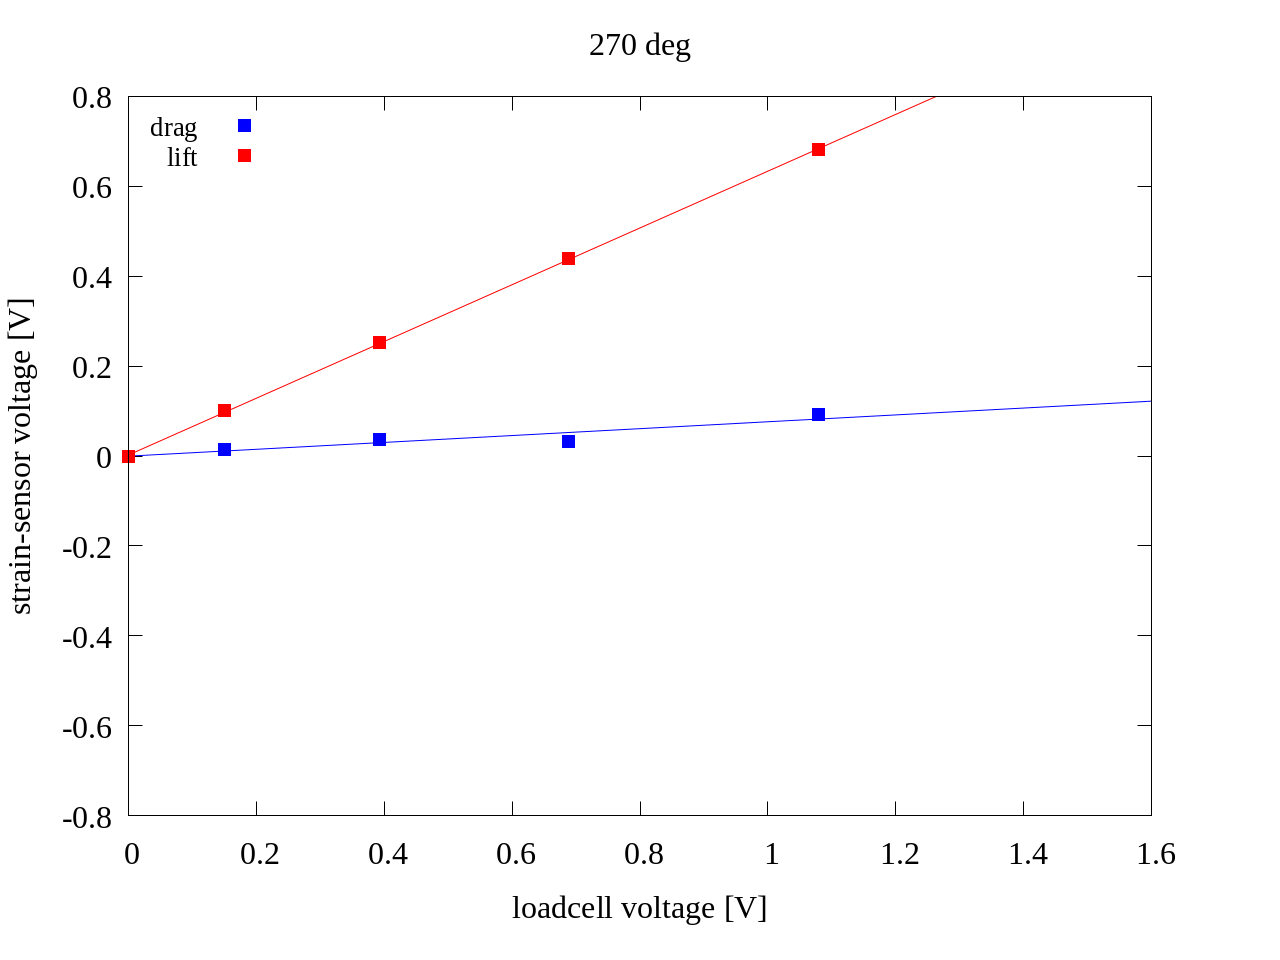
\includegraphics[width=78mm]{../images/linear/270_linear.png}
        \caption{270 deg}
        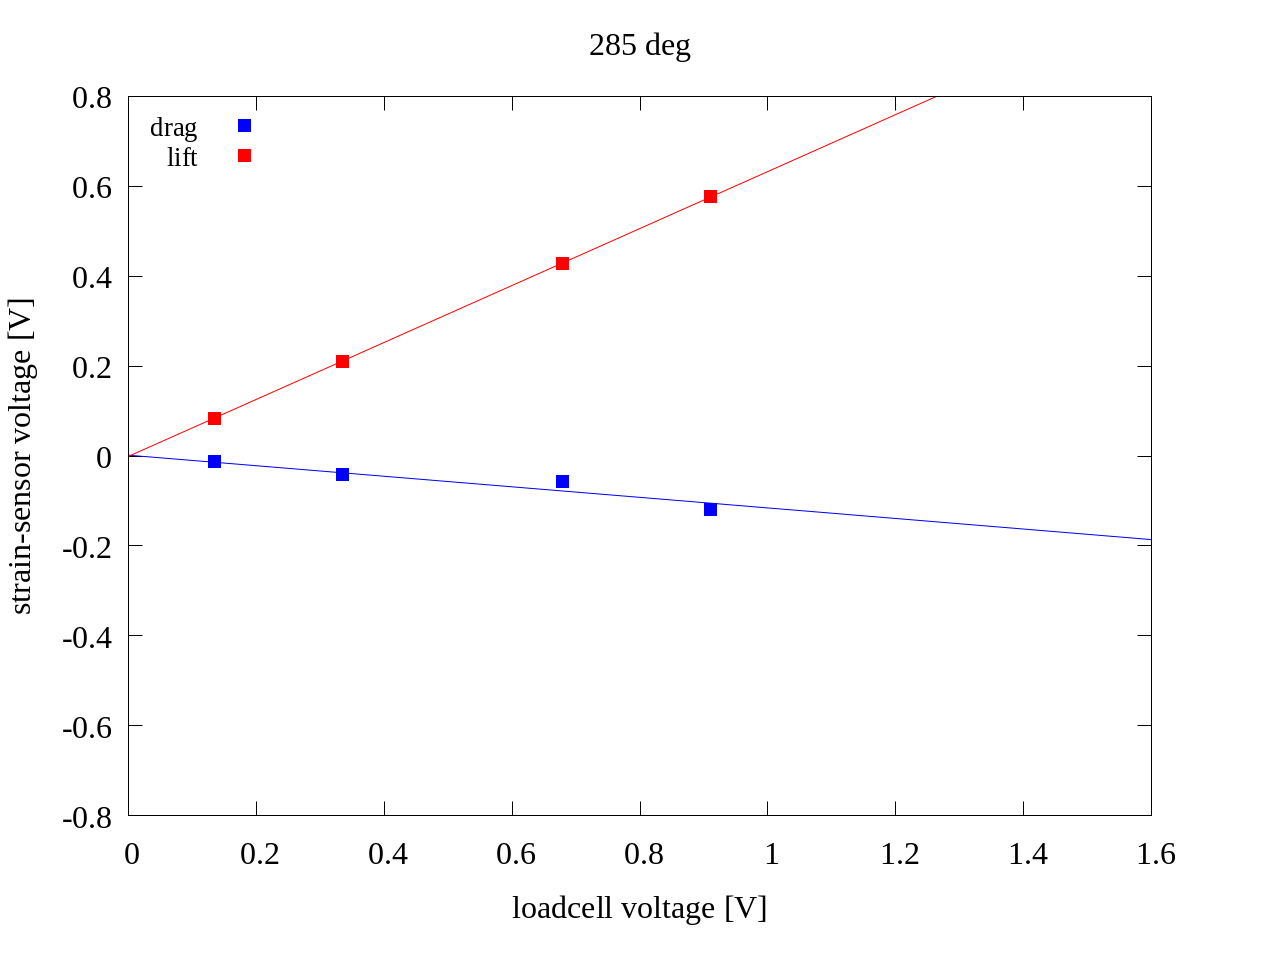
\includegraphics[width=78mm]{../images/linear/285_linear.png}
        \caption{285 deg}
    \end{center}
\end{figure}

\begin{figure}[htbp]
    \footnotesize
    \begin{center}
        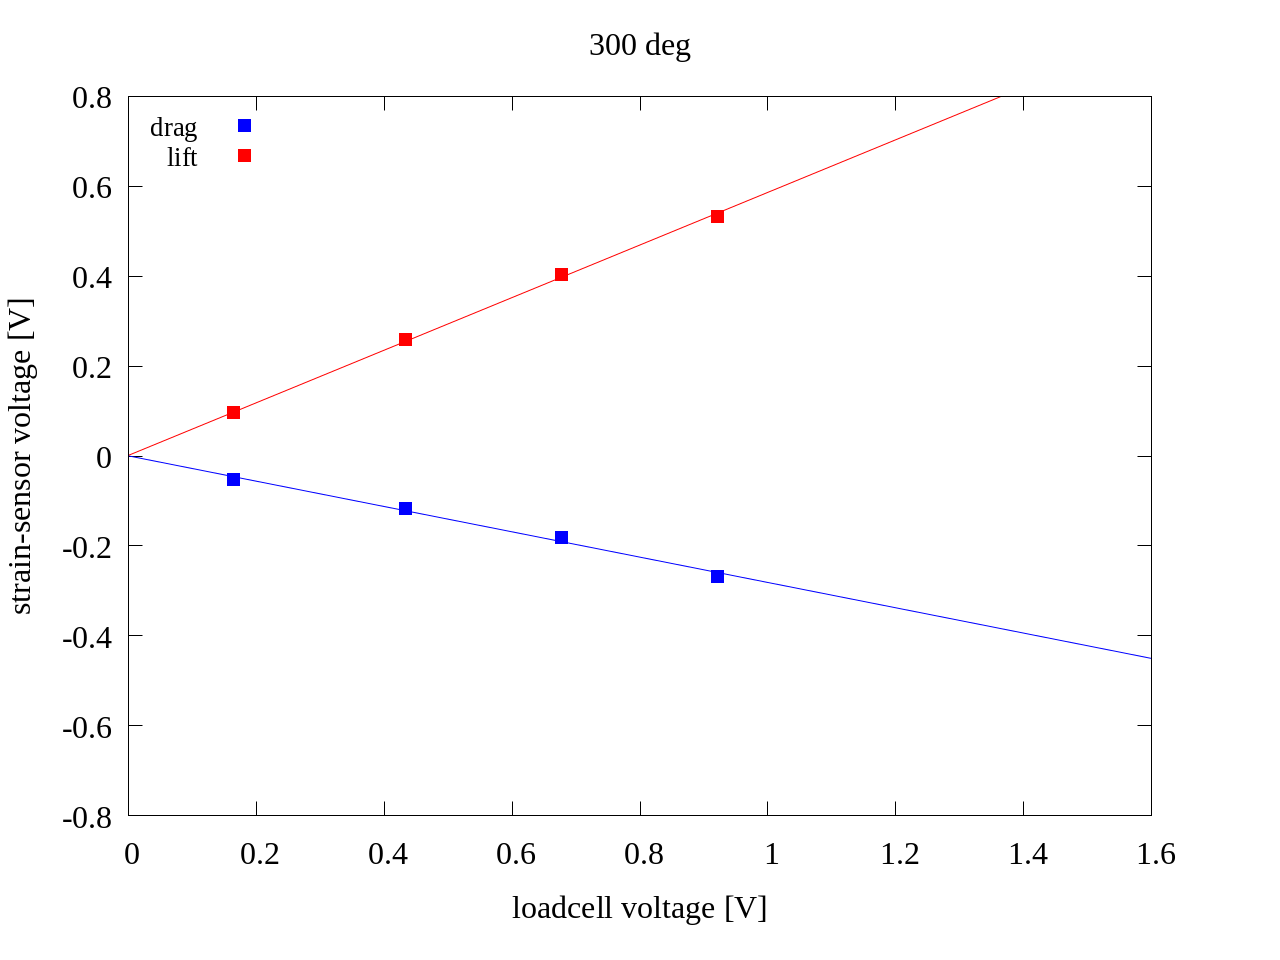
\includegraphics[width=78mm]{../images/linear/300_linear.png}
        \caption{300 deg}
        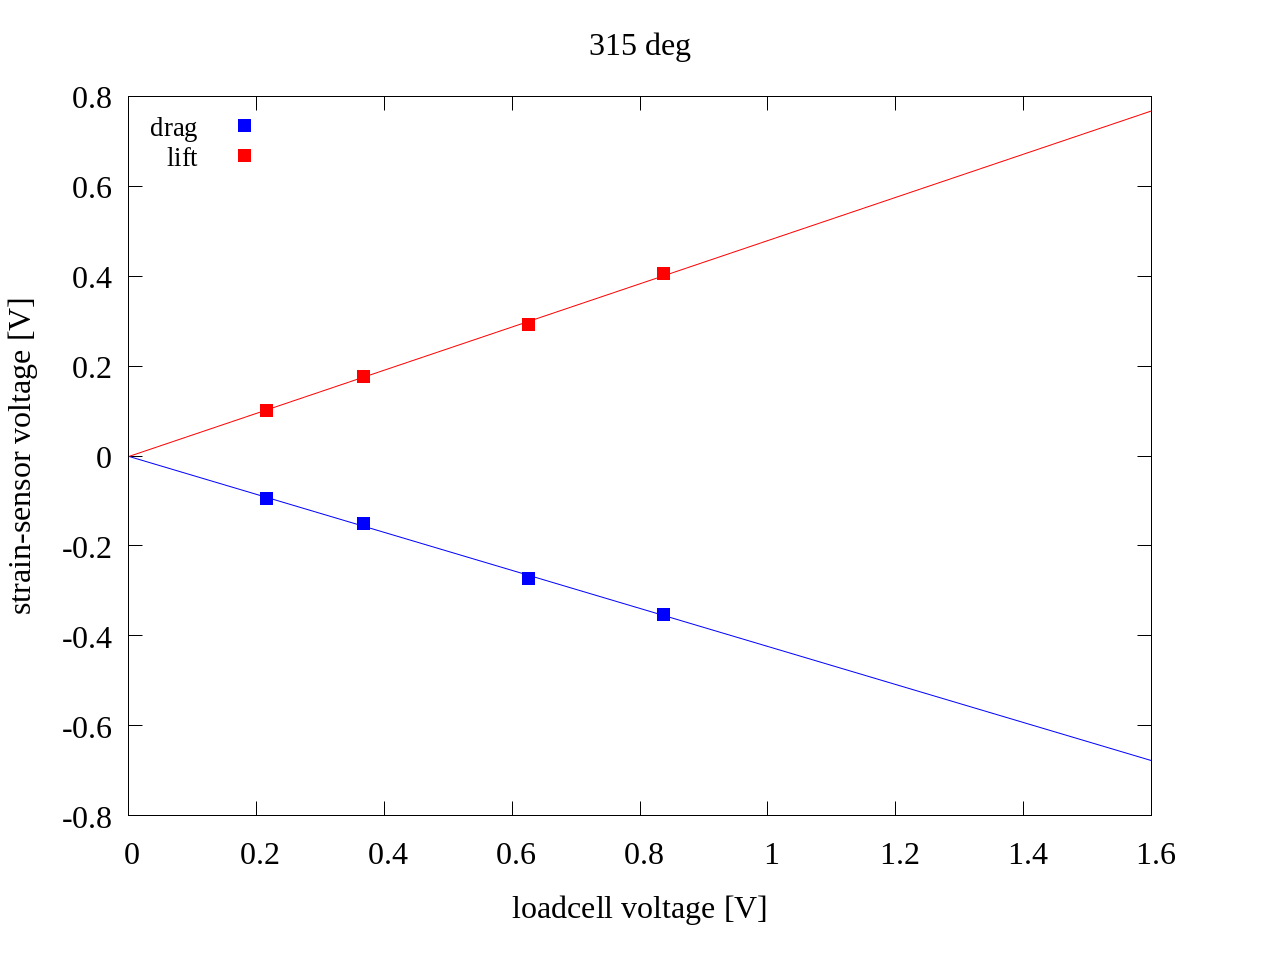
\includegraphics[width=78mm]{../images/linear/315_linear.png}
        \caption{315 deg}
        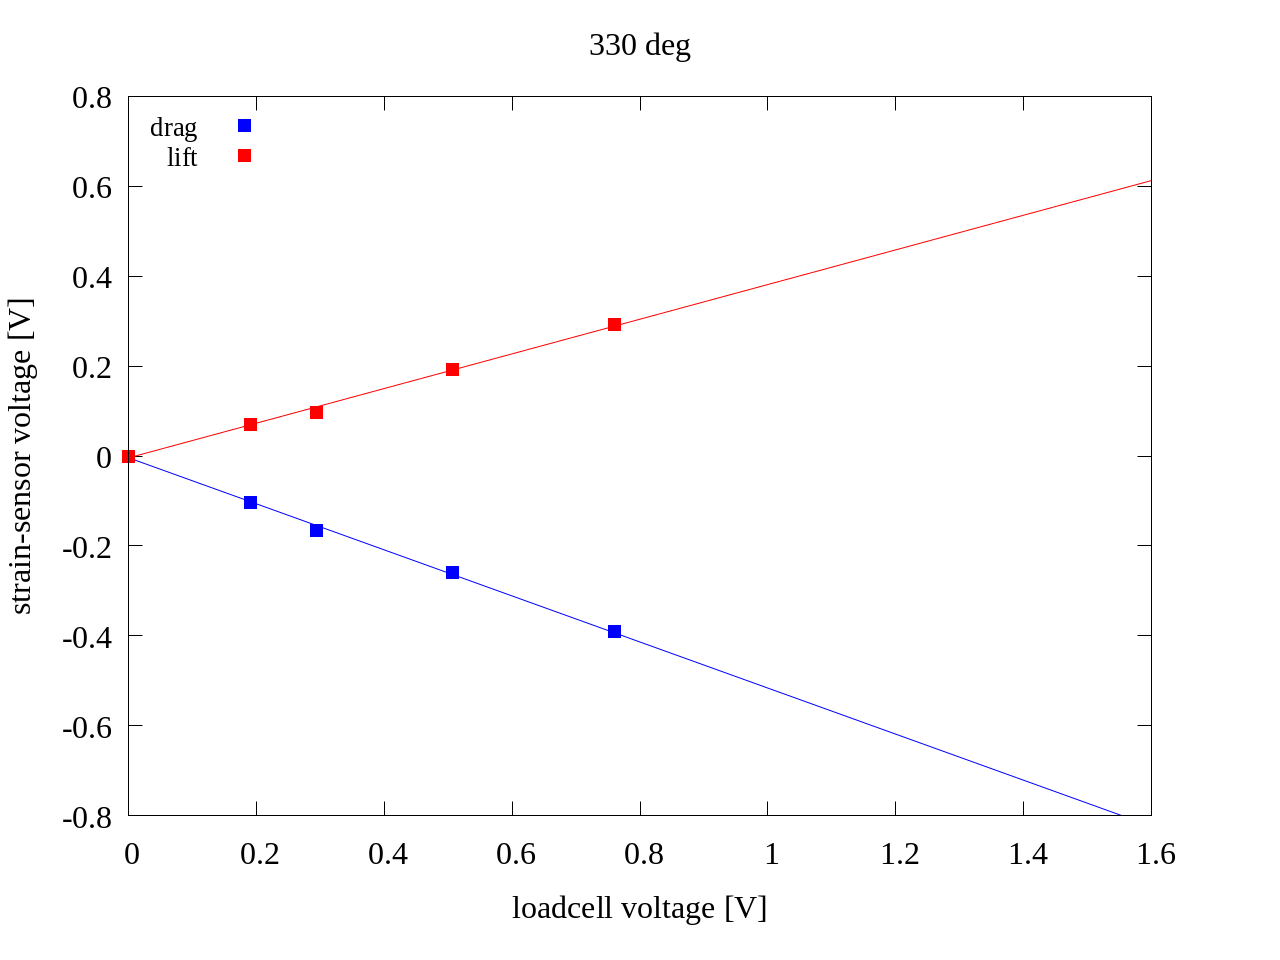
\includegraphics[width=78mm]{../images/linear/330_linear.png}
        \caption{330 deg}
        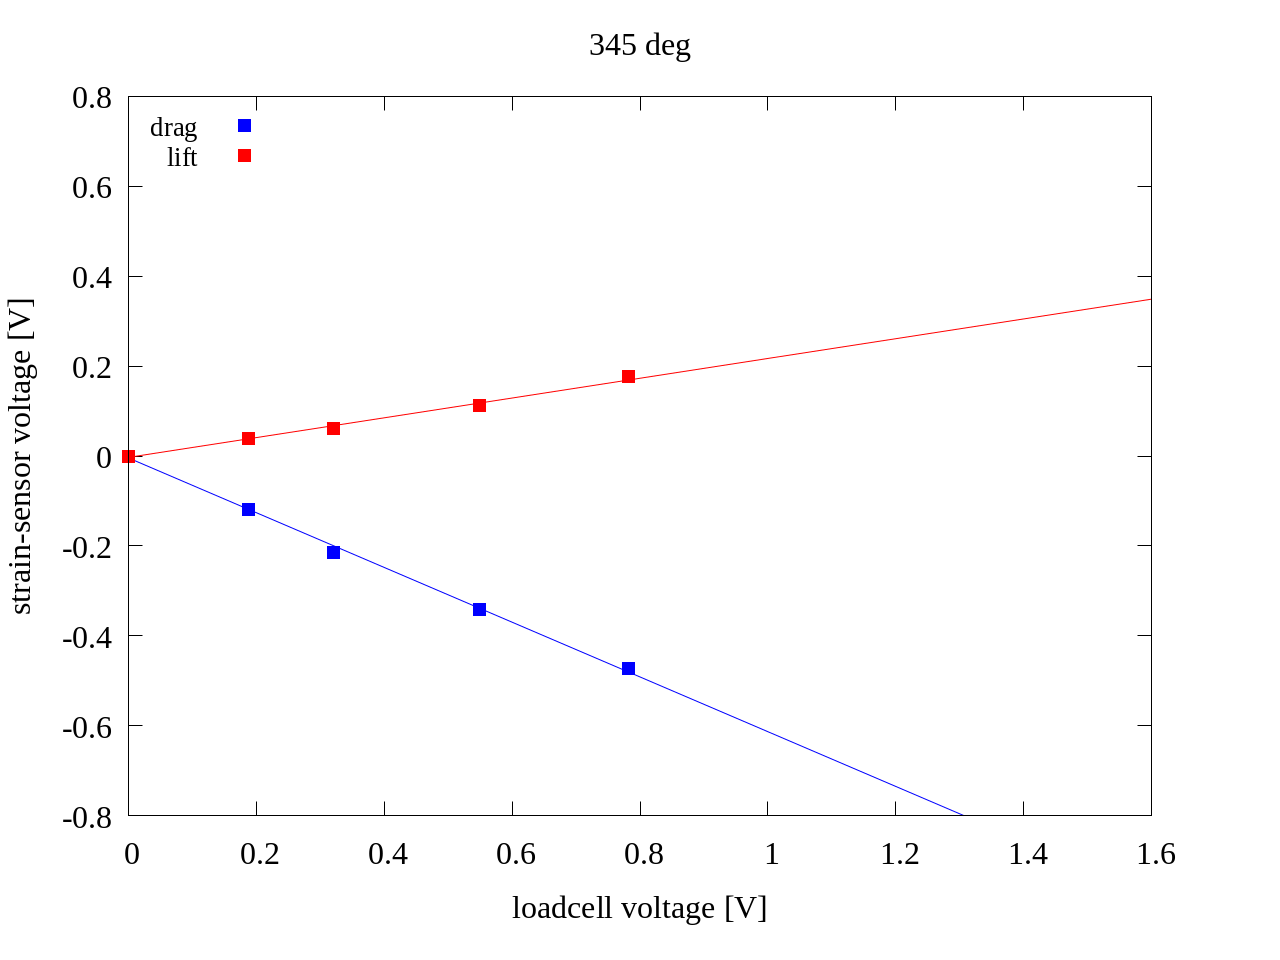
\includegraphics[width=78mm]{../images/linear/345_linear.png}
        \caption{345 deg}
    \end{center}
\end{figure}

\end{document}